% WACV 2024 Paper Template
% based on the CVPR 2023 template (https://media.icml.cc/Conferences/CVPR2023/cvpr2023-author_kit-v1_1-1.zip) with 2-track changes from the WACV 2023 template (https://github.com/wacv-pcs/WACV-2023-Author-Kit)
% based on the CVPR template provided by Ming-Ming Cheng (https://github.com/MCG-NKU/CVPR_Template)
% modified and extended by Stefan Roth (stefan.roth@NOSPAMtu-darmstadt.de)

\documentclass[10pt,twocolumn,letterpaper]{article}

%%%%%%%%% PAPER TYPE  - PLEASE UPDATE FOR FINAL VERSION

\usepackage[T1]{fontenc}    % use 8-bit T1 fonts
%\usepackage[review,algorithms]{wacv}      % To produce the REVIEW version for the algorithms track
%\usepackage[review,applications]{wacv}      % To produce the REVIEW version for the applications track
%\usepackage{wacv}              % To produce the CAMERA-READY version
\usepackage[pagenumbers]{wacv} % To force page numbers, e.g. for an arXiv version


% It is strongly recommended to use hyperref, especially for the review version.
% hyperref with option pagebackref eases the reviewers' job.
% Please disable hyperref *only* if you encounter grave issues, e.g. with the
% file validation for the camera-ready version.
%
% If you comment hyperref and then uncomment it, you should delete
% ReviewTempalte.aux before re-running LaTeX.
% (Or just hit 'q' on the first LaTeX run, let it finish, and you
%  should be clear).
\usepackage[pagebackref,breaklinks,colorlinks]{hyperref}


% Include other packages here, before hyperref.
\usepackage{graphicx}
\usepackage{amsmath}
\usepackage{amssymb}
\usepackage{booktabs}
\usepackage{comment}


\usepackage{url}            % simple URL typesetting
\usepackage{amsfonts}       % blackboard math symbols
\usepackage{nicefrac}       % compact symbols for 1/2, etc.
\usepackage{microtype}      % microtypography
\usepackage{lipsum}         % Can be removed after putting your text content
\usepackage[numbers]{natbib}
\usepackage{doi}

%% extra
\usepackage{listings}
\usepackage{amsmath} 
\usepackage{xcolor}

% Support for easy cross-referencing
\usepackage[capitalize]{cleveref}
\crefname{section}{Sec.}{Secs.}
\Crefname{section}{Section}{Sections}
\Crefname{table}{Table}{Tables}
\crefname{table}{Tab.}{Tabs.}

\newcommand{\cotwo}{\ensuremath{\mathrm{CO_2}}}


%%%%%%%%% PAPER ID  - PLEASE UPDATE
\def\wacvPaperID{*****} % *** Enter the WACV Paper ID here
\def\confName{WACV}
\def\confYear{2025}


\begin{document}

\title{ShitSpotter --- A Dog Poop Detection Algorithm and Dataset}

\author{Jonathan Crall\\
Kitware\\
{\tt\small jon.crall@kitware.com}
%{\tt\small erotemic@gmail.com}
% For a paper whose authors are all at the same institution,
% omit the following lines up until the closing ``}''.
% Additional authors and addresses can be added with ``\and'',
% just like the second author.
% To save space, use either the email address or home page, not both
%\and
%Second Author\\
%Institution2\\
%First line of institution2 address\\
%{\tt\small secondauthor@i2.org}
}
\maketitle

\begin{comment}
    cd $HOME/code/shitspotter
    python -m shitspotter.cli.coco_annotation_stats $HOME/data/dvc-repos/shitspotter_dvc/data.kwcoco.json \
        --dst_fpath $HOME/code/shitspotter/coco_annot_stats/stats.json \
        --dst_dpath $HOME/code/shitspotter/coco_annot_stats
\end{comment}

%%%%%%%%% ABSTRACT
\begin{abstract}

%This work chronicles one researcher's un-funded journey to build a phone
%application that can detect dog poop in images, and make the data widely
%available as a benchmark dataset.
We introduce a new --- currently 42 gigabyte --- "living" dataset of phone images of
dog poop with manually drawn or AI-assisted polygon labels.
The collection and annotation of this data started in late 2020 and is planned
to continue indefinitely.

The most recent snapshot of dataset is made publicly available across three
different distribution methods: one centralized and two decentralized (IPFS and
BitTorrent).
We perform an analysis and observational comparison of the trade-offs between
distribution methods and discuss the feasibility of each with respect to
sharing open scientific data.

A baseline vision transformer is trained to segment the objects of interest
under a grid of hyperparameters, and we evaluate their impact. The best model
achieves a pixelwise mean average precision of ~0.8ish. 
Model weights are made publicly available with the dataset. 

Code to reproduce experiments is hosted on GitHub.

%A phone application to detect poop with these models is being developed and 
%will be made freely available.

\end{abstract}

%%%%%%%%% BODY TEXT
\section{Introduction}
\label{sec:intro}

Applications of a computer vision system able to detect and localize poop in
images are numerous.
Automated waste disposal to keep parks and backyards clean.
A part of a system for using feces to monitor wildlife populations.
A warning system in smart-glasses to prevent people from stepping in poop.
The motivating use case is to develop a phone application that can help a dog
owner find their dog's poop in a leafy park so they can pick it up.
Many of these applications can be realized with modern object detection and
segmentation methods (cite modern object detection and segmentation methods)
and a large labeled dataset to train on.


In addition to enabling several applications, poop detection is an interesting benchmark problem. 
It it a reasonable simple problem with a narrower scope (just a single class),
suitable for exploring the capabilities of object detection models that focus
on a single labeled class while also containing non-trivial challenges like:
resolution (quality of camera, distance to the camera),
distractors (leafs, pine cones, dirt and mud),
occlusion (bushes, overgrown grass),
variation in appearance (old, new, healthy, sick).
Investigation into cases where this problem is difficult may provide insight
into how to better train object detection and segmentation networks.


\begin{figure}[h]
\centering
\includegraphics[width=0.49\textwidth]{figures/viz_three_images.jpg}
\caption[]{
    The "before/after/negative" process.
    The orange box highlights the location of the poop (note the
    actual annotation is a polygon) in the "before" image.
    In the "after" image, it is the same scene but the poop has been removed.
    The "negative" image is a nearby similar scene, potentially with a distractor.
}
\label{fig:ThreeImages}
\end{figure}

Towards these ends we introduce a dataset suitable for training poop detection
models in order to enable applications that require detecting or localizing
poop in images. In order to allow to assist with annotation we collect images
using a "before/after/negative" protocol as shown in \Cref{fig:ThreeImages}. 

Our goal is to train an algorithm to classify which pixels contain poop, and
which don't. We train a segmentation model to provide a baseline on how
difficult this problem is. Our models show strong performance, although there
are notable failure cases indicating this problem is difficult even for modern
computer vision algorithms.

In order to allow other researchers to improve on our results the dataset must
be accessible and at least one entity needs to be willing to host it.
Centralized methods are the typical choice and offer very good speeds, 
but they can be expensive for an individual, so it usually requires an
institution willing to host or payment for a hosting service,
can prone to outages and version control is not built in.
In contrast, decentralized methods allow volunteers to host data offers ability
to validate data integrity. 
This motivates us to compare and contrast centralized cloud services,
BitTorrent, and IPFS as mechanisms for distributing datasets.

% VGG2 face got removed.
% https://github.com/ox-vgg/vgg_face2/issues/52


Our contributions are:
1. A challenging new \textbf{open dataset} of images with polygon segmentations.
2. An experimental \textbf{evaluation of baseline training} methods.
3. An observational \textbf{comparison of dataset distribution} methods.
4. \textbf{Open code and models}.
Related work is discussed at the end.


\section{Dataset}

Our first contribution is the collection of a new open dataset consisting of
dog poop images in a mostly urban environment. The subject matter is primarily
derived from three specific dogs. Indoor images and poop from other dogs are
present in the dataset but were encountered less often and thus are less
frequent.

In addition to this description, details covering the motivation, composition,
collection, preprocessing, uses, distribution, and maintenance are provided in
a standardized datasheet \cite{gebru_datasheets_2021}.

\subsection{Dataset Collection Protocol}
The majority of the dataset was collected using the "before/after/negative"
protocol.
When we encountered a poop in the wild --- usually from our own dogs, but
sometimes from other dogs --- before we dispose of it we 
take a "before" picture containing the poop.
Then we pick up the poop and take an "after" picture of the same area. 
Then we find a nearby area or perhaps something else in the nearby environment
that might act as a confuser (e.g. pine cone or leaf) and take a third
"negative" picture.

The majority of images in the dataset follow this pattern.
However, there are exceptions.
The first 6 months of data collection only involved the "before/after" part of the protocol.
Sometimes the researcher failed or was unable to take the 2nd or 3rd image.
These cases where the before / after / negative protocol can be
programmatically this can be identified.

Additionally, the dataset also contains a few dozen (84) images contributed
by friends and family. These images are images mostly do not follow the
before/after protocol and are marked for use only in testing.


Challenges

\subsection{Dataset Annotation}

Images were annotated using labelme \cite{wada_labelmeailabelme_nodate}. 
The boundaries of 4386 annotated polygons are illustrated in \Cref{fig:AllPolygons}.
Most annotations were initialized using the Segment Anything Model (SAM)
\cite{kirillov_segment_2023} and a point prompt. 
All AI polygons were manually reviewed. In most cases only small manual
adjustments were needed, but there were a significant number of cases where SAM
did not work well and fully manual annotations were needed.
Regions with shadows seemed to cause SAM the most trouble, but there were other
failure cases. Unfortunately, there is no metadata to indicate which polygons
were manually created or done using AI.  However, the number of vertices may be
a reasonable proxy to estimate this, as polygons generated by SAM tend to have
higher fidelity boundaries. 

%Anecdotal note: SAM \cite{kirillov_segment_2023} worked well to automatically
%segment the poop, many of these needed adjustments, especially in regions of
%shadows, but there were cases that required a completely manual approach.
%Unfortunately a clean record of what cases these were does not exist. 

\begin{figure}[h]
\centering
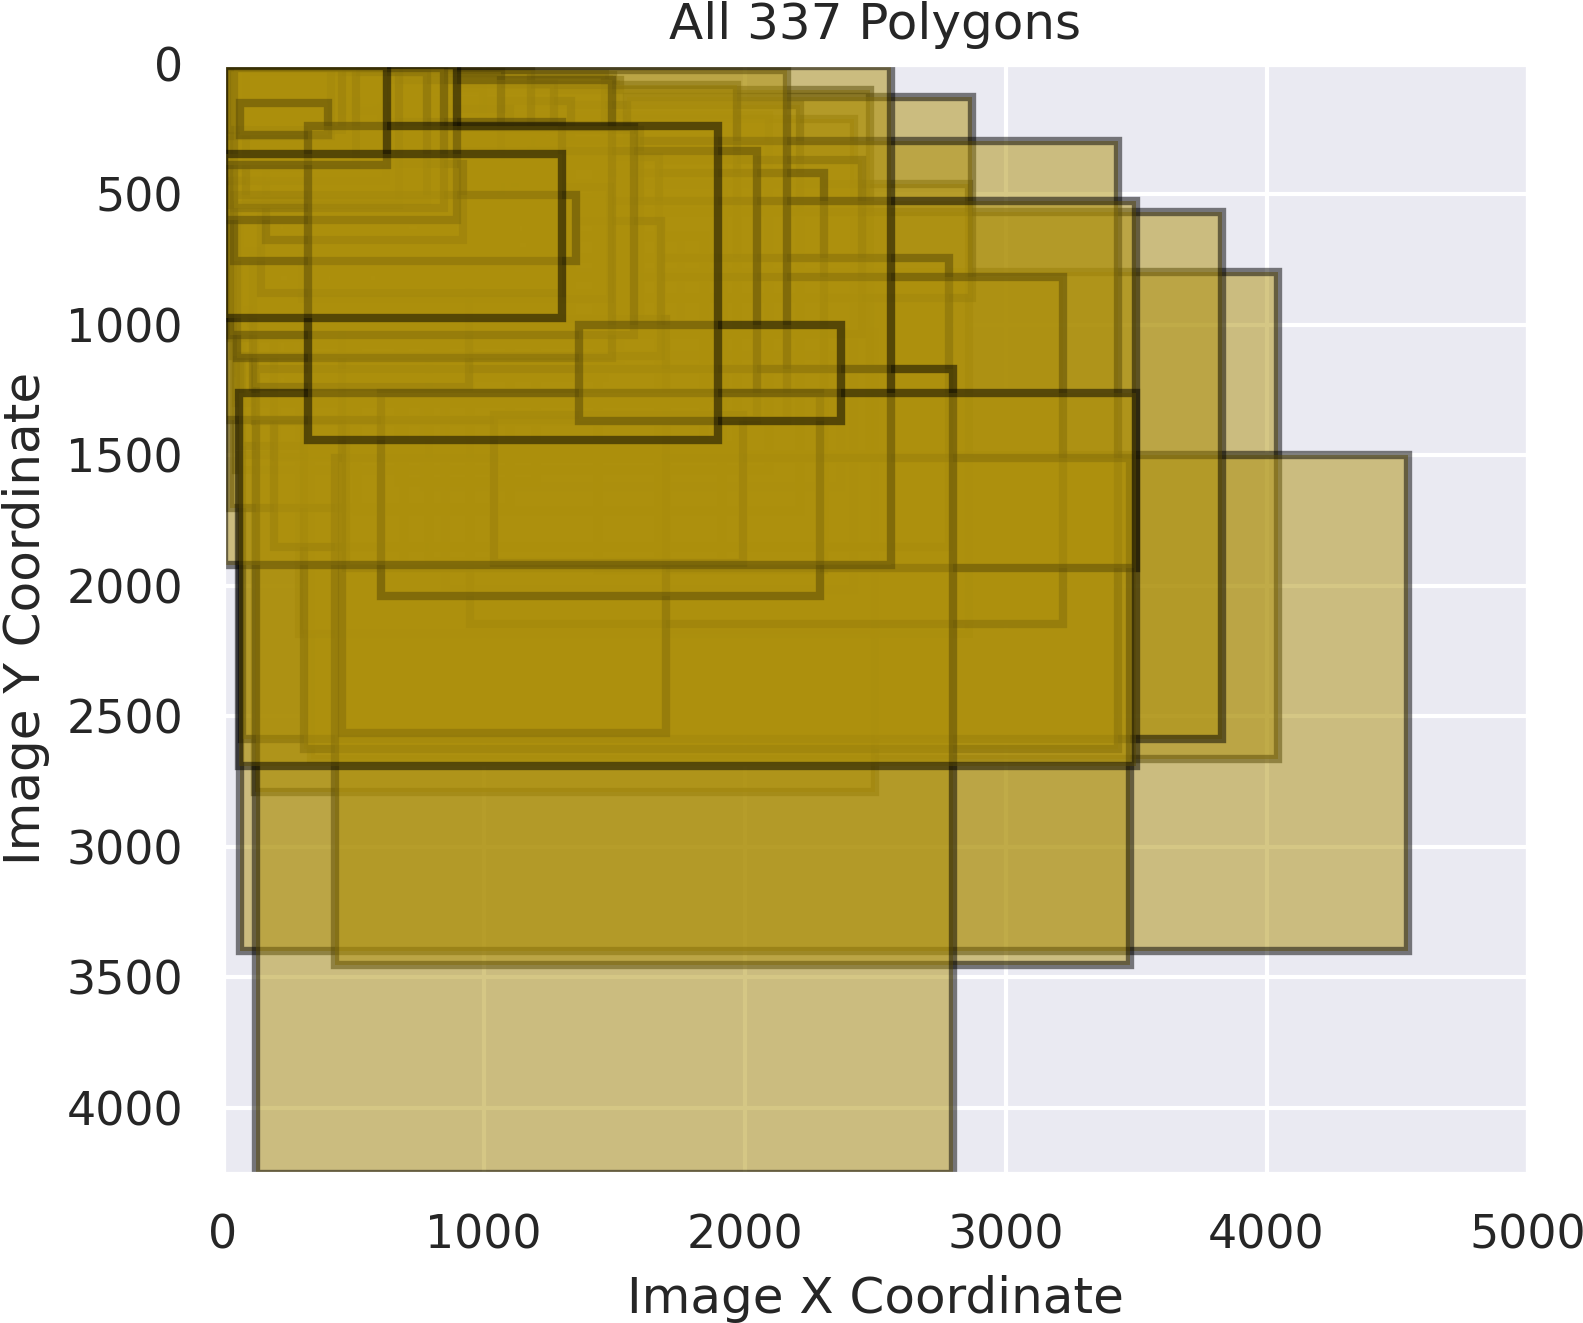
\includegraphics[width=0.4\textwidth]{figures/all_polygons.png}
\caption[]{
    All polygon annotations drawn in a single plot with 0.8 opacity to
    demonstrate the distribution in annotation location, shape, and size with
    respect to image coordinates. Annotations drawn with AI
    assistance tend to have more curved boundaries than manually drawn ones
    (several examples of manual annotations with more jagged boundaries can be
    seen in the top left).
}
\label{fig:AllPolygons}
\end{figure}

\begin{figure}[h]
\centering
\includegraphics[width=0.4\textwidth]{figures/images_timeofday_distribution.png}
\caption[]{
    Scatterplot of the time-of-year vs time-of-day each image was taken.  For
    images with geolocation and timestamp (assuming the timezone is local or
    given and correct) we also estimate the amount of daylight as indicated by
    the color of each dot. While the majority of the images are taken in
    daylight, there are a sizable number of nighttime images.
}
\label{fig:TimeOfDayDistribution}
\end{figure}


\begin{figure}[h]
\centering
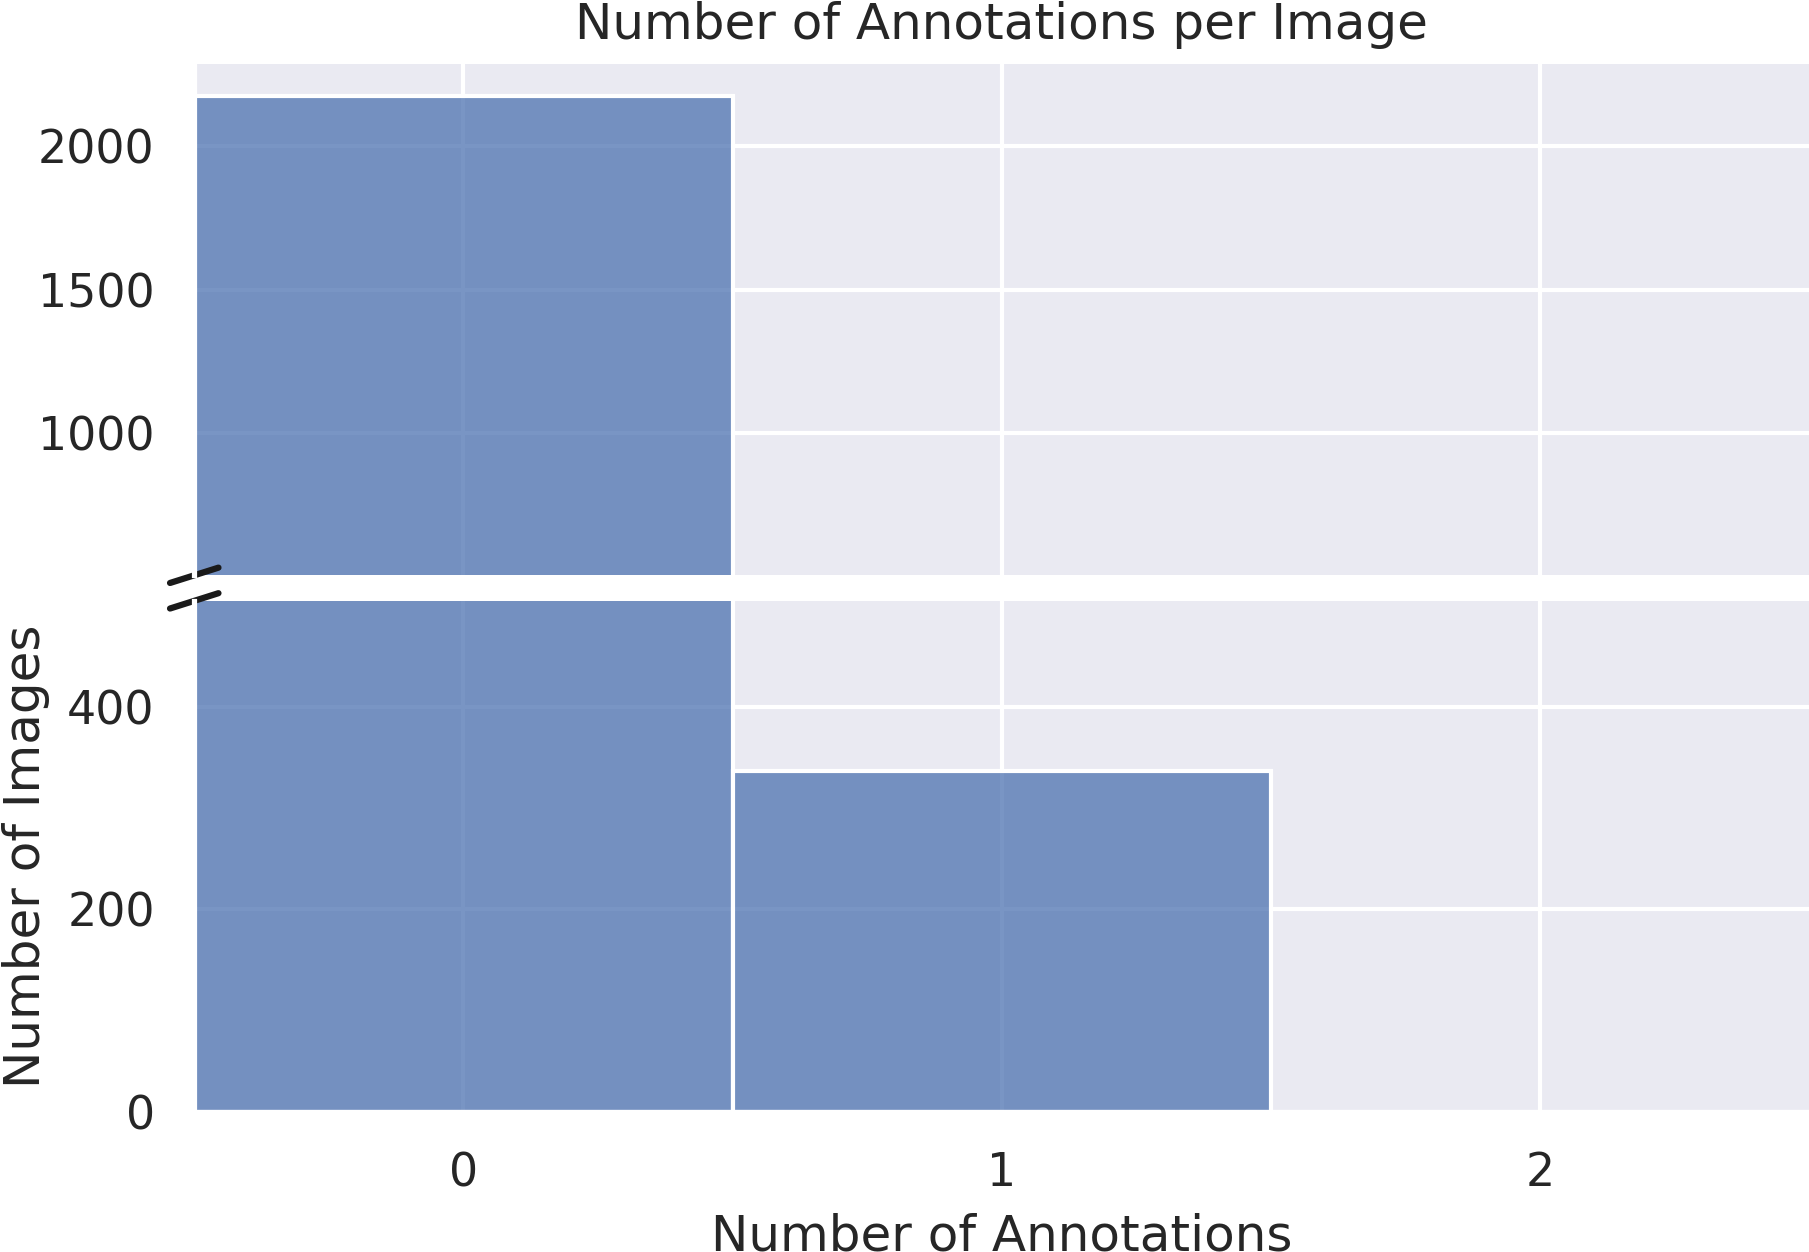
\includegraphics[width=0.4\textwidth]{figures/anns_per_image_histogram_splity.png}
\caption[]{
    Histogram of the number of annotations per image. 
    Only 35\% (2346) of the images contain annotations, the other 65\% (4302)
    are known not to contain poop. Of these 4302 about half of them were taken
    directly after the poop was picked up, and the other half are pictures of a
    nearby location.
}
\label{fig:AnnotsPerImage}
\end{figure}


\begin{figure}[h]
\centering
\includegraphics[width=0.4\textwidth]{figures/spectra.png}
\caption[]{
    The "spectra" or histogram of the pixel intensities in the dataset. 
    The dataset rgb  mean/std is $[117, 124, 100], [61, 59, 63]$ (for reference
    the imagenet mean/std is $[124, 116, 104], [58, 57, 57]$).
}
\label{fig:spectra}
\end{figure}

\subsection{Dataset Stats and Analysis}

% Number of images, annotations, and other stats.

The dataset currently contains 6648 images and 4386 annotations and has spanned
4 years. Data was captured over 4 years at a mostly uniformly rate.  Most data
is localized to parks and sidewalks in a small city.  Weather conditions varied
between snowy, sunny, rainy.  The distribution of seasons, time-of-day,
daylight, and capture rate is illustrated in \Cref{fig:TimeOfDayDistribution}.

Roughly 1/3 of the dataset has annotations due to the other 2/3 of the
images being taken in a way where the object of interest was removed from the
scene.

Some images contain more than one annotation, and some images contain zero annotations.
The number of annotations per images is illustrated in \Cref{fig:AnnotsPerImage}.
Many images do contain more than one poop, and this can be for several reasons:
    1. a single poop broke into multiple disjoint parts (the exact criteria for this is sometimes ambiguous), 
    2. two dogs pooped nearby each other (this happens frequently). 
    3. one or more dogs has pooped in the same area over some period of
       time (some cases can be difficult to determine if it is poop or dirt).

Almost all images have a width/height of 4032 x 3024 (which could be rotated
based on EXIF data) with 6 being 4008 x 5344 and one being 768 x 1024.


\section{Models}

Our second contribution is an evaluation of several trained models to serve as
a baseline.

We use the training and evaluation system of \cite{Greenwell_2024_WACV}, which
can be trained to predict heatmaps from polygons and can evaluate those
heatmaps on a pixelwise-level. 


Specifically, we use the file named train\_imgs5747\_1e73d54f.kwcoco.zip with
5747 images to train and vali\_imgs691\_99b22ad0.kwcoco.zip which contains 691
images is our experimental test set.
In this paper we do not make use of the contributor data


The baseline architecture is a variant \cite{bertasius2021space,Greenwell_2024_WACV} of a vision-transformer \cite{dosovitskiy_image_2021}.

\begin{comment}
geowatch model_stats /home/joncrall/data/dvc-repos/shitspotter_expt_dvc/training/toothbrush/joncrall/ShitSpotter/runs/shitspotter_scratch_20240618_noboxes_v7/lightning_logs/version_1/checkpoints/epoch=0089-step=122940-val_loss=0.019.ckpt.pt
\end{commend}

Number of parameters: 25,543,369.
Memory at train time: ~20GB
Memory at predict time: 1.961GB.
Model size on disk: 114.19 MB.

Rate of patches on 3090 with 1 background worker: 20.93Hz
GPU hits 94% utilization at predict time.

In all experiments, we use half-resolution images, which means most images have
an effective width/height of 2016 x 1512. The network is given a widow size of
416,416, which means that multiple windows are needed to predict on entire
images.

Our model is a 12 layer encoder backbone with 384 channels, and 8 attention
heads. 
The segmentation head is a 4 layer MLP using encoder features.
Loss is computed pixelwise using FocalLoss \cite{ross2017focal} with a small
downweighting of pixels towards the edge of the window.
The optimizer is AdamW, and we vary learning rate, weight decay, and
perturb-scale (note: weight decay combined with a non-zero perterb scale
implements the shrink perturb trick: \cite{ash_warm_starting_2020}).
We use a OneCycle learning rate scheduler with a cosine annealing strategy and
starting fraction of 0.3.
Our effective batch size is 24 with a real batch size of 2 and 12 accumulate
gradient steps.


All regions without an annotation were available at train time, but we used an
undersampling strategy to randomly choose equal numbers of negative windows as
there were positive windows (i.e. windows with annotations in them).

This used about 20-22 GB of the 24 GB available on the 3090 throughout
training.

%\textbf{Static Parameters}:

\subsection{Model Experiments}

\begin{comment}
    SeeAlso:
    ~/code/shitspotter/experiments/run_pixel_eval_pipeline.sh

    python ~/code/shitspotter/dev/poc/estimate_train_resources.py
\end{comment}

Our experiments are meant mean to provide a reasonable baseline, and not a
comprehensive evaluation of state of the art models on this dataset.

Exact scripts to reproduce these experiments are in the code repo.

After finding a reasonable performing starting point, we performed an ablation
over learning rate and regularization parameters. 
\begin{figure}[h]
\centering

\includegraphics[width=0.4\textwidth]{figures/macro_results_resolved_params.heatmap_pred_fit.trainer.default_root_dir_metrics.heatmap_eval.salient_AP_vs_metrics.heatmap_eval.salient_AUC_PLT02_scatter_nolegend.png}%
(a)
\includegraphics[width=0.4\textwidth]{figures/macro_results_resolved_params.heatmap_pred_fit.trainer.default_root_dir_metrics.heatmap_eval.salient_AP_PLT04_box.png}%
(b)
\caption[]{
    (a) A scatterplot of the pixelwise AP and AUC of the top-5 checkpoints evaluated on the validation set.
    For each training run we ran evaluation on a subset of checkpoints that
    achieved low validation loss.
    Points with the same color represent checkpoints from the same training run
    with with the same hyperparameters.

    (b) The range of AP values over the top-5 checkpoints evaluated on the validation set.
    TODO: link this to the table of parameters

    \Cref{tab:parameters_and_results} provides more details about the maximum
    AP points per run.
}
\label{fig:apauc_scatter}
\end{figure}


%\begin{figure}[h]
%\centering
%\includegraphics[width=0.4\textwidth]{figures/macro_results_resolved_params.heatmap_pred_fit.trainer.default_root_dir_PLT05_table.png}
%\caption{
%    The table mapping short names to the default root directory.
%    TODO: create a table that shows an overview of the varied hyperparameters.
%}
%\label{fig:scatter_legend}
%\end{figure}

% Scatterplot for all experiments used in this work.
% file:///home/joncrall/data/dvc-repos/shitspotter_expt_dvc/_shitspotter_evals/full_aggregate/plots/macro-plots-macro_01_c1edce/params/resolved_params.heatmap_pred_fit.trainer.default_root_dir/scatter_nolegend/macro_results_resolved_params.heatmap_pred_fit.trainer.default_root_dir_metrics.heatmap_eval.salient_AP_vs_metrics.heatmap_eval.salient_AUC_PLT02_scatter_nolegend.png


\begin{table*}[t]
\centering
\begin{tabular}{llllrr}
\toprule
                       default\_root\_dir &      lr & weight\_decay & perterb\_scale &  salient\_AP &  salient\_AUC \\
\midrule
scratch\_20240618\_v7 &  0.0001 &     0.000001 &      0.000003 &    0.8325&     0.9927\\
scratch\_20240618\_v6 &  0.0001 &          0.0 &           0.0 &    0.8225&     0.9795\\
scratch\_20240618\_v5 &  0.0001 &      0.00001 &           0.0 &    0.8203&     0.9678\\
scratch\_20240618\_v4 &  0.0001 &     0.000001 &           0.0 &    0.8159&     0.9872\\
scratch\_20240618\_v2 &  0.0003 &     0.000003 &      0.000001 &    0.8107&     0.9685\\
scratch\_20240618\_v3 &   0.001 &      0.00001 &      0.000003 &    0.7665&     0.9899\\
scratch\_20240618\_v8 &  0.0001 &     0.000001 &           0.0 &    0.7458&     0.9662\\
\bottomrule
\end{tabular}
\caption{
    Scores for the best top model on the validation set for each of the 7 hyperarameter configurations. These correspond to the maximum AP 
    of each run in \Cref{fig:apauc_scatter}.
}
\label{tab:parameters_and_results}
\end{table*}


This restricted of the top-5 checkpoints per training run is illustrated in \Cref{fig:apauc_scatter} and details for the best checkpoint and hyper-parameters are given in \Cref{tab:parameters_and_results}.

We evaluate each model with standard pixelwise segmentation metrics, where each
pixel is is considered as a binary classification example (poop-vs-background).
For each pixel the truth is compared to its predicted score, and we compute
standard metrics of average-precision (AP) and  area under the ROC curve (AUC)
\cite{powers_evaluation_2011}.

\Cref{fig:parameters_and_results} illustrates the AP and AUC of all baseline models trained.
These include ad-hoc parameters settings when searching for a stable training
configuration.


We trained 7 models from scratch with varied hyperparameters.

All models were trained on a single machine with an 11900k CPU and a 3090 GPU.

We measure the predict-time resources using codecarbon \cite{lacoste2019codecarbon} and report them in 
\Cref{tab:resources}.


% See: ./scripts/estimate_training_resources.py
Handling these measurements at train time is still in development, but we
estimate the time of each training run using timestamps on checkpoint and log
files.  Using indirect measurements based on timestamps of log and checkpoint
files, we estimate that each of the 7 training runs took about 5 days and 15
hours, totaling about 49.2 GPU days. Using the maximum 350W power draw of a
3090 GPU, we estimate energy usage of 17.2 kilowatt hours, assuming a 0.21
conversion ratio is 3.6 kilograms of CO2.


However, the experiments presented here were not the only ones performed in
determining the hyperparameters we held constant here. 

The path to the presented experiments involved trying over 42 training run with
a wider variation of parameters. In total we estimate the total GPU time as
158.9 days with an average of 3.75 days per run, which is emits roughly 280.4
\cotwo{} kg with a cost of about \$4.21 to offset.

\subsubsection{Results}

\begin{figure*}[h]
\centering
\includegraphics[width=1.0\textwidth]{figures/test_heatmaps_with_best_vali_model}%
\hfill
(a) test set
\includegraphics[width=1.0\textwidth]{figures/vali_heatmaps_with_best_vali_model.jpg}%
\hfill
(b) validation set
\includegraphics[width=1.0\textwidth]{figures/train_heatmaps_with_best_vali_model.jpg}%
\hfill
(c) training set
\caption[]{
    Qualitative results using the highest scoring model on the validation set
    on a selection of images from (a) the test test, (b) the validation set and
    (c) the training set.
    Success cases are on the left, and failures increase towards the right.
    %
    In each figure, the top rows shows true positive pixels in white, false
    positive pixels in red, false negative pixels in teal, and true negative
    pixels in black.  For visualization purposes, the threshold to binarize the
    prediction is chosen to maximize the F1 for each image, thus the top row is
    in some sense the best possible classification of the heatmap, which is
    shown in the middle row. The final row is the input image.
    %
    Most images in the (small, 30 image) test set are qualitatively good.
    Failure cases are limited to close up images of older sometimes
    partially-deteriorated poops.

    These examples were manually selected and ordered by hand. (could recompute
    the order based on some measure).
}
\label{fig:test_heatmaps_with_best_vali_model}
\end{figure*}


Qualitative results for the test, validation, and training set are shown in
\cref{fig:test_heatmaps_with_best_vali_model}. These examples illustrate
success and failure cases. The test and validation set both show clear
responses to the objects of interest. 

Notably the much larger training set also contains errors. This indicates that
there is still more information that can be extracted from this dataset,
perhaps with hard mining techniques.

Even though focal loss was used, the current learning curriculum is likely
under weighting smaller distant objects. Our pixelwise evaluation metric is
biased against it, which is a current limitation.

There are clear difficult cases in certain sticks, leafs, and dark areas on
snow.



\begin{table}[t]
    \centering
\begin{tabular}{llllr}
\toprule
        node & resource &           total &            mean &  num \\
\midrule
eval & time & 07:52:02 &  00:13:29 &   35 \\
pred & time & 04:23:34 &  00:07:32 &   35 \\
pred &   co2\_kg &        0.6678&         0.0191 &   35 \\
pred &      kwh &        3.1729&        0.0907&   35 \\
\bottomrule
\end{tabular}

(a)

\begin{tabular}{llllr}
\toprule
        node & resource &           total &            mean &  num \\
\midrule
eval & time & 4 days 14:37:02 & 00:20:07 &  330 \\
pred & time & 6 days 06:52:11 & 00:27:31 &  329 \\
pred &   co2\_kg &       17.9547&        0.0546 &  329 \\
pred &      kwh &       85.3051&        0.2599 &  329 \\
\bottomrule
\end{tabular}

(b)

\label{tab:resources}
\caption[]{
Time and energy resources used to perform model evaluation.

The pred node is the heatmap prediction step in the pipeline.
The eval node is the pixelwise evaluation step in the pipline. 

(a) resources used in the presented evaluations.
(b) resources used in hyperparameter tuning beforehand.

Note: this table does not include training time, which was not measured
directly at the time. Our stated train time estimates are based on.

}
\end{table}


\section{Open Data Distribution}

% BitTorrent can be vulnerable to MITM:
% https://www.reddit.com/r/technology/comments/1dpinuw/south_korean_telecom_company_attacks_torrent/

Our third contribution is an exploration and observational study of distributed
and centralized data distribution methods. 

Advantages of content addressability:
* reproducibility 

There is a well known reproducibility "crisis" in science \cite{baker_reproducibility_2016}.

Even in computer science, success rates at reproducing the results of others ~60%
\cite{NEURIPS2019_c429429b, collberg2016repeatability, desai_what_2024}.

We believe that reducing friction in accessing the data may help improve the
success rate. This involves codifying data download and preparation. Datasets
that are content addressable are ideal for this because they avoid the issue of
dead urls.

However, there is a drawback. The time to connect to peers can be substantial
if the data does not have many "seeders". 


Cloud storage for a modest amount of data can be expensive.

Decentralized methods can allow information to persist so long as at least 1
person has the data.

BitTorrent is a well known distributed system.

IPFS is a new similar tool \cite{benet_ipfs_2014,bieri_overview_2021}.


Both BitTorrent (as of 2017 in the v2 protocol \cite{cohen_bittorrent_2017})
and IPFS can recognize that two torrents/CID include the same file and seeders
can provide files to downloaders of the other.

Discuss distributing the dataset via IPFS versus centralized distribution
systems.

%Decentralized Method - IPFS and BitTorrent.
%Centralized Method - Girder

The specific version of the dataset used in this paper was snap-shotted on
2024-07-03 and has the IPFS content ID of:
bafybeiedwp2zvmdyb2c2axrcl455xfbv2mgdbhgkc3dile4dftiimwth2y.
% https://academictorrents.com/docs/about.html
Dataset is tracked on Academic Torrents \cite{academic_torrents_Cohen2014}.


IPFS vs BitTorrent:

IPFS is fully content addressable.
BitTorrent is partially content addressable.

Both of which have the ability to use the Kademlia - distributed hash table (DHT) \cite{maymounkov_kademlia_2002}.
IPFS always uses its DHT, where as BitTorrent the Kademlia-based Mainline
Tracker can be disabled in favor of 3rd party trackers.

An excellent overview of protocols details can be found \cite{zebedee_comparing_2023}.
Our comparison is going to focus on measurements.
% Overview and comparison of protocols via github gist:
% https://gist.github.com/liamzebedee/224494052fb6037d07a4293ceca9d6e7
% https://gist.github.com/liamzebedee/4be7d3a551c6cddb24a279c4621db74c
%[Steiner, En-Najjary, Biersack 2022]
% See Also:
% Long Term Study of Peer Behavior in the KAD DHT
% https://git.gnunet.org/bibliography.git/plain/docs/Long_Term_Study_of_Peer_Behavior_in_the_kad_DHT.pdf
% We have been crawling the entire KAD network once a day for more than a year to track end-users with static
% IP addresses, which allows us to estimate end-user lifetime and the fraction of end-users changing their KAD ID.




\subsection{Distribution Observations}

To assess the effectiveness of distributed distribution of datasets, we perform
an observational study. We attempt to download the dataset via each of the 3
primary distribution mechanisms, and measure the time it takes to complete.
For distributed methods, there wasn't a clear automated mechanism to measure
lag-time for connecting to peers, which was a significant issue in these tests.

As an example centralized distribution mechanism we use the Girder
\cite{girder_2024} data management platform.
For bittorrent we use the transmission-client \cite{transmission_2024}.
For IPFS we use the standard kubo implementation \cite{girder_2024}.
We also include direct "rsync" \cite{rsyncprojectrsync_2024} between machines as a baseline method.

A difference between the girder and decentralized methods is that the former
required that the data was packaged into separate zip files, which could
improve transfer efficiency due to fewer file boundaries.

In all tests, the source and destination machines are separated by about 30
kilometers with an average ping time of 48.480ms. For each test we create a
measurement log (included in supplemental materials) and record the start
time and end time of the transfer. We also include notes and command line
invocations.

The average durations between the start of the transfer command and its
completion are shown in \cite{tab:transfertime}.

\begin{table}[t]
\begin{tabular}{llllll}
\toprule
{} & count &   mean &    std &   min &    max \\
method        &       &        &        &       &        \\
\midrule
bittorrent & 3 & 11.41 & 4.00 & 6.87 & 14.39 \\
ipfs & 3 & 4.14 & 2.13 & 1.80 & 5.96 \\
rsync & 2 & 4.60 & 2.12 & 3.10 & 6.10 \\
girder & 1 & 1.33 & - & 1.33 & 1.33 \\
\bottomrule
\end{tabular}
\label{tab:transfertime}
\caption[]{
    Number of hours of transfer speeds of entire dataset averaged of n trials,
    noted in the "count" column. 
}
\end{table}


In addition to these measurements we have made several anecdotal observations
that are worth discussing.

\begin{itemize}
    \item IPFS via https using gateways does not always work well.
    \item IPFS usually works well if you use the CLI.
    \item IPFS is easier to update.
    \item IPFS does rehash every file, which induces an O(N) scalability constraint.

    \item BitTorrent and IPFS seem to both take awhile to establish connection
          to a peer when there are a small number of pinners/seeders.

          IPFS has a mechanism to directly connect to a peer, which seems to
          work fairly quickly, but not immediately.

          This issue is mitigated as the number of seeders/pinners grows.
          A test download of ImageNet LSVRC 2017 dataset from academic torrents
          almost immediately connected to 2 seeders.

    \item Centralized solutions depend on an organization providing a service,
          and that organization can choose to stop providing that service.
\end{itemize}



%-------------------------------------------------------------------------
\section{Related Work}


The ImageNet dataset \cite{ILSVRC15}.

The MSCOCO dataset \cite{lin_microsoft_2014}.

Object detection

Waste detection is an important problem but with relatively few open datasets.
%  https://paperswithcode.com/dataset/zerowaste
The ZeroWaste dataset \cite{bashkirova_zerowaste_2022} contains 1,800 segmented
video frames and 6000 unlabeled frames in a recycling facility.
% https://paperswithcode.com/dataset/taco
The TACO dataset \cite{proenca_taco_2020} is another "living" dataset
containing 1500 images with 4,784 annotations over 60 classes.
% TrashCan https://paperswithcode.com/dataset/trashcan
% Top Datasets on paperwith code
% https://paperswithcode.com/datasets?mod=images&task=semantic-segmentation&page=2


% Domestic Trash / Garbage Dataset
% Looks like the full dataset is behind a paywall
% https://paperswithcode.com/dataset/domestic-trash-garbage-dataset


% https://universe.roboflow.com/dataset-vmyna/poop-yxidr/dataset/1
% 102 train images, 22 validation images, 0 test images.
% human poop


While ours is the largest publicly available poop dataset that we are aware of,
it is not the first.
A dataset of 100 dog poop images was collected and used to train a FasterRCNN
model in 2019 but this dataset and model are not publicly available \cite{neeraj_madan_dog_2019}.
The MSHIT dataset \cite{mshit_2020} consists of 3.89GB of real images with fake
poop (e.g. plastic poop) in controlled environments.
The company iRobot has a dataset of annotated indoor poop images used to train
Roomba j7+ to avoid collisions, but as far as we are aware, this is not
available \cite{roomba_2021}.


IPFS and BitTorrent are the distributed distribution mechanism we consider, but there are others

% Very good overview and comparison of the protocols
% https://blog.mauve.moe/posts/protocol-comparisons
% https://distributed.press/
% hypercore - https://github.com/tradle/why-hypercore/blob/master/FAQ.md#how-is-hypercore-different-from-ipfs
% git,
% Secure Scuttlebut (SSB)

\section{Conclusion}

The ShitSpotter dataset is 42GB of images with polygon segmentations of dog
poop. 

We train and evaluate several baseline segmentation models, the best of which 
achieve an AP/AUC of ...

Our dataset is sufficient to train an object detection network to (level of
precision/recall).
Our experimental evaluation is limited by lack of model diversity, but it
serves as a baseline for future exploration.

We make data and models available over 3 distribution mechanisms: 
cloud storage, BitTorrent, and IPFS.

Decentralized methods are feasible methods of distribution, with strong
security but they can be slow.
IPFS is a promising solution for hosting scientific datasets, but does have pain points.
In contrast bittorrent can do X/Y/Z, but ...
Lastly centralized cloud storage can give the best speeds, but sacrifices some
security and can be less robust.

Directions for future research / development are:
1. Add lightweight object-level head and test object detection metrics.
2. Optimize model architectures for mobile devices.
3. Launch phone application.
4. Improve model / data distribution.


%%%%%%%%% REFERENCES
{\small
\bibliographystyle{ieee_fullname}
\bibliography{citations}
}
%\bibliographystyle{unsrtnat}
%\bibliography{references}  %%% Uncomment this line and comment out the ``thebibliography'' section below to use the external .bib file (using bibtex) .


\begin{comment}
    cd $HOME/code/shitspotter
    python -m shitspotter.cli.coco_annotation_stats $HOME/data/dvc-repos/shitspotter_dvc/data.kwcoco.json \
        --dst_fpath $HOME/code/shitspotter/coco_annot_stats/stats.json \
        --dst_dpath $HOME/code/shitspotter/coco_annot_stats

    SeeAlso:
    ~/code/shitspotter/experiments/run_pixel_eval_pipeline.sh
    ~/code/shitspotter/experiments/run_pixel_eval_on_test_pipeline.sh
    ~/code/shitspotter/experiments/run_pixel_eval_on_train_pipeline.sh

    python ~/code/shitspotter/dev/poc/estimate_train_resources.py

    See: ./localize_figures.sh


    Best Validation Model:
        /home/joncrall/data/dvc-repos/shitspotter_expt_dvc/training/toothbrush/joncrall/ShitSpotter/runs/shitspotter_scratch_20240618_noboxes_v7/lightning_logs/version_1/checkpoints/epoch=0089-step=122940-val_loss=0.019.ckpt.pt
        # Best Rank:  33.0 pyzvffmyjcrq
        Lives in /home/joncrall/data/dvc-repos/shitspotter_expt_dvc/_shitspotter_test_evals/eval/flat/heatmap_eval/heatmap_eval_id_0f613533/pxl_eval.json heatmap_eval           pyzvffmyjcrq    0.505110     0.912509
        

    Best Test Model:
        /home/joncrall/data/dvc-repos/shitspotter_expt_dvc/training/toothbrush/joncrall/ShitSpotter/runs/shitspotter_scratch_20240618_noboxes_v6/lightning_logs/version_0/checkpoints/epoch=0073-step=101084-val_loss=0.017.ckpt.pt
        is Rank 3 on the validation dataset.
    

    cd /home/joncrall/code/shitspotter/shitspotter_dvc
    geowatch spectra --src data.kwcoco.json --workers=16 --cache_dpath=_spectra_cache --dst spectra.png --bins 64 --valid_range=0:255
    cp spectra.png ~/code/shitspotter/papers/application-2024/figures/spectra.png


\end{comment}

\end{document}
